\documentclass[preprint, 11pt]{article}

\usepackage[T1]{fontenc}
\usepackage[utf8]{inputenc}
\usepackage[hmargin=0.9in, vmargin=1.25in]{geometry}
\usepackage[babel]{csquotes}
\usepackage{subfig}
\usepackage{graphicx}
\usepackage[colorlinks=true,citecolor=blue,urlcolor=blue]{hyperref}
\usepackage{caption}
\usepackage{amsmath}          % writing mathematical formulas
\usepackage{amsthm}           % writing mathematical theorems
\usepackage{amssymb}          % writing mathematical symbols
\usepackage{bm, amsfonts}     % writing bold mathematical symbols
\usepackage{xcolor}
\usepackage{fixmath}
\usepackage{tikz}
\usepackage{bm}
\usepackage{makecell}
\usepackage{mathdots}
\usepackage{algpseudocode}
\usepackage{algorithm}

\newcommand{\W}{{\mathcal W}}
\newcommand{\A}{{\mathcal A}}
\newcommand{\apdq}{\A^+ \!\!{\Delta} Q}
\newcommand{\amdq}{\A^- \!\!{\Delta} Q}
\newcommand{\Ft}{\tilde{F}}
\newcommand{\imh}{{i-1/2}}
\newcommand{\iph}{{i+1/2}}
\newcommand{\bff}{{\bf f}}
\newcommand{\bfr}{{\bf r}}
\newcommand{\bfF}{{\bf F}}
\newcommand{\bfu}{{\bf u}}
\newcommand{\bfv}{{\bf v}}
\newcommand{\bfq}{{\bf q}}
\newcommand{\bfx}{{\bf x}}
\newcommand{\sgn}{{\rm sgn}}
\newcommand{\Rus}{{\rm Rus}}
\newcommand{\Roe}{{\rm Roe}}

%\newdefinition{rmk}{Remark}
\newtheorem{remark}{Remark}

\title{Numerical simulation and entropy dissipative cure of the
  carbuncle instability for the shallow water circular hydraulic jump}

\author{
    David I. Ketcheson \and
    Manuel Quezada de Luna
}
\begin{document}

\maketitle

\begin{abstract}
We study numerical discretizations of the shallow water equations
for the simulation of the circular hydraulic jump formed
when a vertical fluid jet impacts a horizontal plate.
This is a challenging problem that includes a curved steady shock
that can be physically unstable.  We show that numerical methods are prone to
either suppress the instability completely or form artificial carbuncles.
We test existing cures for the carbuncle as well as a new method,
and show results that exhibit the shock instability without unphysical carbuncles.
\end{abstract}



\section{Introduction}

\subsection{The circular hydraulic jump}

Perhaps the first reference to the observation of the circular hydraulic jump
comes from Lord Rayleigh \cite{rayleigh1914theory}, who wrote that it
``may usually be seen whenever a stream of water from a tap strikes a horizontal
surface".  This phenomenon that is familiar in the everyday kitchen sink, is in
fact highly nonlinear and complex.  Near the jet, the flow is shallow and
supercritical, while further away it is deeper and subcritical.  The transition from supercritical
to subcritical flow
occurs in a very narrow region and takes the form of a \emph{jump} or \emph{bore}
that is roughly circular if the surface is flat; we refer to it herein as a
circular hydraulic jump (CHJ).

Early experimental work on the CHJ began some time later
\cite{kurihara1946hydraulic,tani1949water,watson1964radial}.
Watson \cite{watson1964radial} derived the jump radius
implied by Rayleigh's approach and the vertical
velocity profile in the supercritical region, assuming a no-slip
boundary condition at the bottom.  He also studied the turbulent
flow case and performed experiments.
More detailed experiments revealed different qualitative classification
of jumps  \cite{ishigai1977heat,craik1981circular}.
Although later work incorporated more physical details (such as surface tension) into the models
\cite{bush2003influence}, Bohr et. al. showed that important properties of the jump
(particularly its radius) could be reasonably predicted using a simple shallow water
model \cite{bohr1993shallow}.

While the jump is roughly circular, under appropriate conditions it may deviate
from this shape and deform rapidly and chaotically in time.
Instability of the jump was observed from fairly early on \cite{craik1981circular}.
Under special circumstances with more viscous fluids, the jump instability may lead to
the formation of curious shapes such as polygons \cite{ellegaard1998creating}, but
for a low-viscosity fluid like water the behavior is generally chaotic.
The strength of the instability increases with the jet velocity and with the
depth at the outside of the jump.  For fluids with finite viscosity, the flow
can also be completely steady for sufficiently small velocities and depths.


\subsection{Numerical shock instabilities}

In \cite{peery1988blunt} a numerical instability was observed to
appear near the symmetry plane in the simulation of a bow shock.
This phenomenon, subsequently dubbed ``carbuncle", has been observed by many researchers
in similar numerical experiments for the Euler equations, and many remedies
have been proposed, mainly in the form of additional numerical dissipation
\cite{quirk1997contribution,pandolfi2001numerical,dumbser2004matrix,chauvat2005shock,ismail2009proposed,shen2014stability}.
Most notably, the HLLE Riemann solver suppresses the carbuncle instability \cite{quirk1997contribution}.
For a recent review of numerical shock instability and work to alleviate it,
we refer to \cite[Section 2.5]{simonnumerical}.

Given the similarity of structure between the Euler equations and the shallow
water equations, it is not surprising that carbuncles appear in numerical
solutions of the latter as well \cite{kemm2014note}.
The shallow water carbuncle behaves similarly to the
Euler carbuncle: it appears when the Roe solver is used, but not when
the HLL solver is used, and can be suppressed by similar numerical methods
\cite{kemm2014note,bader2014carbuncle}.

As we will see, carbuncles also appear in the numerical solution of the shallow
water circular hydraulic jump.  This is natural, since the solution involves a
standing shock wave.  Dealing with the carbuncle in this context is particularly
interesting and challenging, since this standing shock should (at least in an
appropriate flow regime) be unstable, and some research has suggested that the
carbuncle is the manifestation of a true physical
instability \cite{moschetta2001carbuncle,elling2009carbuncle}.




\begin{itemize}
  \item Describe the carbuncle instability starting with Euler and going to SWEs.
  \item Mention that we observe the cc instability for the CHJ as well.
  \item Describe that in this case, the situation is more complicated than in other problems since we
    expect the correct solution to have physical instabilities triggered by round off error.
  \item Based on existing literature we know that we can use highly dissipative and robust methods to
    avoid the formation of carbuncle instabilities. However, in this case, these methods also tend to
    dissipate other important features of the solution unless the mesh is highly refined.
  \item We are interested in methods that prevent the formation of cc instability in the CHJ
    but preserve other features and physical instabilities.
  \item There are multiple ideas and methods proposed to fix the cc insitability for the Euler
    and recently for the SWEs.
  \item It is believed that the cc instability occurs due to lack or reduced viscosity in the shear contact waves.
  \item Some methods also propose to improve the entropy stability properties of the method. In particular, to induce or guarantee that the entropy is dissipated at shocks.
  \item Based on some of these ideas we start with Rusanov's method using the cell averages of the solution.
    This is a first-order method that is entropy stable and positivity preserving. We enhance its robustness by
    overestimating the wave speed when strong shear is present in the solution. The result is a robust solver
    that do not develop cc instabilities. However, the method is highly dissipative and, as a result,
    many other important features of the solution are dissipated.
  \item We then blend this highly dissipative method with a FV method based on Roe's average.
  \item After this we introduce the second order corrections from Law-Wendroff's method.
\end{itemize}

\subsection{Our contribution}
\begin{itemize}
\item We present a new problem where the cc instability occurs. In our opinion, this is a more challenging
  problem than the standard bow shock problem since we expect the solution to be non-steady.
  We aim to preserve instabilities that are inherently present in the CHJ for certain regimes. And,
  at the same time, we aim to prevent the cc instability.
\item We explore the use of entropy dissipation and entropy stability as cure of the cc instability for the SWEs.
\item We propose a specific method to blend the highly dissipative and robust Rusanov's RP and the
  accurate 3-wave Roe's solver for the SWEs.
\item We demonstrate that this scheme prevents the formation of cc instabilities not only
  in the well-known bow shock problem, but also in the CHJ while preserving other important features of
  the solution.
\end{itemize}


\section{The shallow water circular hydraulic jump}
We consider the shallow water model in two horizontal dimensions:
\begin{subequations} \label{eq:sw}
\begin{align}
    h_t + (hu)_x + (hv)_y & = 0 \\
    (hu)_t + \left(hu^2 + \frac{1}{2}gh^2\right)_x + (huv)_y & = 0 \\
    (hv)_t + (huv)_x + \left(hv^2 + \frac{1}{2}gh^2\right)_y & = 0.
\end{align}
\end{subequations}
Here $h, u,$ and $v$ are respectively the depth and the $x$- and $y$-components of
velocity, which are functions of the two spatial coordinates $(x,y)$ as well as time $t$.
The gravitational force is proportional to $g$.
%The system \eqref{eq:sw} can be written in vector form as
%\begin{align}
%    q_t + f(q)_x + g(q)_y & = 0.
%\end{align}

\subsection{Semi-analytical steady solution under rotational symmetry}\label{sec:steady_chj}
In this work, we consider the initial boundary value problem consisting of the
shallow water model \eqref{eq:sw} in an annular domain
\begin{align}
r_\textup{jet} \le r \le r_\infty
\end{align}
where $r = \sqrt{x^2+y^2}$, with prescribed inflow at $r=r_\textup{jet}$
and prescribed outflow at $r=r_\infty$.
The domain and boundary conditions are rotationally symmetric.
By assuming rotational symmetry in \eqref{eq:sw}, one obtains the system
\begin{subequations} \label{eq:rsw}
\begin{align}
    (rh)_t + (rhu)_r & = 0 \label{mass1} \\
    (rhu)_t + (rhu^2)_r + r \left(\frac{1}{2}gh^2\right)_r = 0. \label{mom1}
\end{align}
\end{subequations}
where the depth $h$ and radial velocity $u$ are functions of the single spatial coordinate $r$.
Steady-state solutions of \eqref{eq:rsw} satisfy
\begin{subequations}\label{steady}
\begin{align}
    rhu & = C \\
    h'(r) & = \frac{h}{\frac{g}{\beta^2} r^3 h^3 -r} = \frac{h}{r} \cdot \frac{F^2}{1-F^2} \label{eq:dh}
\end{align}
\end{subequations}
for some $C$ independent of $r$.  Here $F=|u|/\sqrt{gh}$ is the Froude number.
We see that two types of steady profiles exist, depending on whether the flow
is subcritical ($|F|<1$) or supercritical ($|F|>1$).  No smooth steady solution can
include both regimes, since the right hand side of \eqref{eq:dh} blows up when $F=1$.

The steady, rotationally-symmetric circular hydraulic jump involves supercritical
flow for $r<r_0$ and subcritical flow for $r>r_0$, where $r_0$ is the jump radius.
The jump itself takes the form of a stationary shock wave.  The Rankine-Hugoniot jump
conditions specify that for such a shock,
\begin{align} \label{eq:RH}
    h_+ - h_- & = \frac{-3h_- + \sqrt{h_-^2 + 8 h_- u_-^2/g}}{2} = \frac{3h_-}{2}\left(\sqrt{1+\frac{8}{9}(F_-^2-1)}-1\right),
\end{align}
where the subscripts $+, -$ denote states just inside or outside the jump radius, respectively.

A steady-state, rotationally symmetric solution can be given for an annular region with prescribed
flow at the inner and outer boundaries as follows:

\begin{enumerate}
    \item Specify the depth and velocity at the inner boundary (near the jet) and outer boundary.
    \item Integrate \eqref{eq:dh} from both boundaries.
    \item Find a radius $r_0$ where the matching condition \eqref{eq:RH} is satisfied.
\end{enumerate}
Due to the nature of solutions of \eqref{eq:dh}, it can be shown that the required jump
radius $r_0$ always exists if the prescribed flow is supercritical at the inner boundary
and subcritical at the outer boundary.

Numerical tests suggest that the solution of \eqref{eq:rsw} tends rapidly approaches that
just described under general initial conditions as long as the flow at the jet is
supercritical and the outer outflow is subcritical.  This solution remains steady
if the rate of inflow and outflow are matched.  The stability of this solution in
the face of non-rotationally-symmetric perturbations is an important question not
only in the shallow water context but for more realistic fluid models and physically.
It will play an important role in the results we present later.
The rotationally-symmetric steady state is a useful initial condition for studies
of CHJ stability.


\section{Numerical methods}
In this work we study the behavior of certain shock-capturing finite volume
methods based on the use of Riemann solvers.  For simplicity, we discuss these
solvers in the context of a 1-dimensional mesh.  
In the numerical experiments in \S\ref{sec:num} we use second-order Strang
splitting \cite{strang1968construction} to extend the method to multiple dimensions.

\subsection{Wave propagation methods}\label{sec:waveprop}
The numerical solution $u_i$
represents the average value over cell $i$, which extends from $x_\imh$ to $x_\iph$.
At each time step and at each interface $x_\imh$, we approximately solve the
Riemann problem with initial states $(u^n_{i-1},u^n_i)$.  The approximate
solution consists of a set of traveling discontinuities or waves $\W^p_\imh$
and corresponding speeds $s^p_\imh$.
We use the wave propagation framework developed by LeVeque \cite{leveque1997wave, leveque2002finite}
and employed in the Clawpack software \cite{clawpack,pyclaw-sisc}, which implements the LWL scheme
\begin{align}\label{second-order_via_fluct}
  u_i^{n+1} = u_i^n-\frac{\Delta t}{\Delta x}\left[\apdq_\imh+\amdq_\iph\right]
  -\frac{\Delta t}{\Delta x}\left[\tilde{F}_{i+1/2}-\tilde{F}_{i-1/2}\right],
\end{align}
Upon defining $z^+:=\frac{1}{2}(z+|z|)$ and $z^-:=\frac{1}{2}(z-|z|)$,
the fluctuations are given by
\begin{align}\label{fluct}
  \apdq_\imh := \sum_p\left(s_{i-1/2}^p\right)^+\W_{i-1/2}^p, \qquad
  \amdq_\iph := \sum_p\left(s_{i+1/2}^p\right)^-\W_{i+1/2}^p, \\
\end{align}
and represent the effect (to first
order accuracy) of waves coming from the solution of the Riemann problem at
each of the neighboring interfaces.  Meanwhile, $\Ft_{i\pm 1/2}$ are correction
fluxes that make the method second-order accurate:
\begin{align*}
  \tilde{F}_{i\pm 1/2}=\frac{1}{2}\sum_p|s_{i\pm 1/2}^p|\left(1-\frac{\Delta t}{\Delta x}|s_{i\pm 1/2}^p|\right)\tilde\W_{i\pm 1/2}^p.
\end{align*}
Here $\tilde{\W}_{i\pm 1/2}^p$ is a TVD-limited version of $\W_{i\pm 1/2}^p$.
We will sometimes work with
the first-order method obtained by setting the correction fluxes to zero:
\begin{align}\label{first-order_via_fluct}
  u_i^{n+1} = u_i^n-\frac{\Delta t}{\Delta x}\left[\apdq_\imh+\amdq_\iph\right]
\end{align}
which, for the conservative Riemann solvers we use herein, can also be written
as a first-order flux-differencing scheme:
\begin{align}\label{first-order_FV}
  \bfu_i^{n+1}=\bfu_i^n-\frac{\Delta t}{\Delta x}\left[\bfF_{i+1/2}-\bfF_{i-1/2}\right],
\end{align}
where $\bfF_{i+1/2}$ is a numerical approximation of the flux at $x_\iph$.

Next we briefly review two commonly-used Riemann solvers: those of Rusanov and
Roe.  Neither of these solvers deals with the carbuncle instability in fully
satisfactory way.  Rusanov's solver suppresses the carbuncle but is known to
also suppress related real instabilities, while Roe's solver exhibits carbuncles.
Later we will combine these two solvers in order to better deal with shock instability.
We refer to \cite{ketcheson2020riemann} and references therein for
a full and detailed description of these two Riemann solvers in the context of
the shallow water equations.  Both of these solvers satisfy the conservation
property
\begin{align} \label{rs_conservation}
    \amdq_\imh + \apdq_\imh = \bff(\bfu_i) - \bff(\bfu_{i-1}).
\end{align}


\subsection{Rusanov's Riemann solver}\label{sec:rusanov}
The Rusanov solver approximates the Riemann solution by with a single wave traveling in each
direction.  Both waves are assumed to travel with speed $\lambda^{\max}_\imh$, which is an
upper bound on the wave speeds appearing in the true solution of the Riemann problem.
In this work, we take $\lambda_{i-1/2}^{\max}$ to be the upper bound
from \cite[Prop. 3.7]{azerad2017well}.
The waves are then given by
\begin{align}\label{rusanov_waves}
  \W_{i-1/2}^{1,\Rus}=\bfu_{i-1/2}-\bfu_{i-1}, \qquad
  \W_{i-1/2}^{2,\Rus}=\bfu_{i}-\bfu_{i-1/2},
\end{align}
where the intermediate state $\bfu_{i-1/2}$ is determined by imposing conservation:
\begin{align}\label{rus_cons}
  -\lambda_{i-1/2}^{\max}\W_{i-1/2}^{1,\Rus}+\lambda_{i-1/2}^{\max}\W_{i-1/2}^{2,\Rus} = \bff(\bfu_{i})-\bff(\bfu_{i-1}).
\end{align}
The fluctuations are given by \eqref{fluct} with $s_{i-1/2}^1=-\lambda_{i-1/2}^{\max}$
and $s_{i-1/2}^2=\lambda_{i-1/2}^{\max}$, and the first- and second-order methods based
on Rusanov's solver are given by \eqref{first-order_via_fluct} and \eqref{second-order_via_fluct}, respectively.


\subsection{Roe's Riemann solver} \label{sec:roe}
The Roe Riemann solver is based on evaluating the flux Jacobian using Roe's average
\begin{align}\label{roe_average}
  \bar h_{i-1/2}=\frac{1}{2}(h_{i-1}+h_i), \qquad
  \hat u_{i-1/2}=\frac{\sqrt{h_{i-1}}u_{i-1}+\sqrt{h_i}u_i}{\sqrt{h_{i-1}}+\sqrt{h_i}}, \qquad
  \hat v_{i-1/2}=\frac{\sqrt{h_{i-1}}v_{i-1}+\sqrt{h_i}v_i}{\sqrt{h_{i-1}}+\sqrt{h_i}}.
\end{align}
The waves and speeds are given by the eigenvectors and eigenvalues of the approximate
flux Jacobian obtained using these averages, resulting in
\begin{align*}
  \hat\lambda_{i-1/2}^1=\hat u_{i-1/2}-g\sqrt{g\bar h_{i-1/2}}, \qquad
  \hat\lambda_{i-1/2}^2=\hat u_{i-1/2}, \qquad
  \hat\lambda_{i-1/2}^3=\hat u_{i-1/2}+g\sqrt{g\bar h_{i-1/2}}. \\
\end{align*}
and $\W_{i-1/2}^p=\alpha_{i-1/2}^p\hat r_{i-1/2}^p$, with
\begin{align*}
  \hat \bfr^1_{i-1/2} =
  \begin{bmatrix}
    1 \\
    \hat u_{i-1/2}-\sqrt{g\bar h_{i-1/2}}\\
    \hat v_{i-1/2}
  \end{bmatrix},
  \qquad
  \hat \bfr^2_{i-1/2} =
  \begin{bmatrix}
    0\\
    0\\
    1
  \end{bmatrix},
  \qquad
  \hat \bfr^3_{i-1/2} =
  \begin{bmatrix}
    1 \\
    \hat u_{i-1/2}+\sqrt{g\bar h_{i-1/2}}\\
    \hat v_{i-1/2}
  \end{bmatrix}
\end{align*}
and the factors $\alpha^p_\imh$ obtained by solving
\begin{align}\label{system_for_alphas}
  \left[\hat \bfr^1_{i-1/2} ~\hat \bfr^2_{i-1/2} ~\hat \bfr^3_{i-1/2}\right]
  \begin{bmatrix}
    \alpha^1_{i-1/2} \\
    \alpha^2_{i-1/2} \\
    \alpha^3_{i-1/2}
  \end{bmatrix}
  =\Delta Q_{i-1/2}:=\bfu_i-\bfu_{i-1}.
\end{align}



\section{An entropy-based blending of Rusanov and Roe}

As we discussed in the introduction, finite volume methods with
Roe's Riemann solvers are prone to the carbuncle instability for the CHJ.
In contrast, if we use Rusanov's
Riemann solver, no carbuncles appear; however, many other important and physical features of
the solution are dissipated, unless the grid is highly refined.
Our main objective is to study the CHJ and to propose a Riemann solver
that is carbuncle-free but does not dissipate important features of the solution.
To do that we propose a Riemann solver that blends Rusanov's and Roe's solvers.
Our blending criterion is based on the residual of the entropy (in)equality,
which induces dissipation of entropy near discontinuities.
Blending these Riemann solvers has been proposed before
to solve the Euler equations, see e.g.
\cite{nishikawa2008very,wang2016developing,jaisankar2007diffusion,ohwada2018simple,deng2019new,ray2013entropy},
the shallow water equations, see e.g. \cite{bader2014carbuncle,kemm2014note},
and even the Navier-Stokes equations, see e.g. \cite{nishikawa2008very,ohwada2018simple}.
In these references, the authors use blending criteria different than ours.
Nevertheless, fixing the carbuncle instability by imposing entropy stability is not new.
For example, in \cite{ismail2009affordable,ismail2009proposed},
the authors developed carbuncle free solvers for the Euler equations
via dissipation of entropy.


%We close this section by remarking that the fluctuations associated with Rusanov's solver
%can be expressed in terms of waves and speeds from Roe's solver. To see this, first consider \eqref{rus_cons}
%and rewrite the right-going fluctuation as follows:
%\begin{align}\label{rus_rs_aux}
%  \A^{+,\Rus}\Delta Q_{i-1/2}:=\lambda_{i-1/2}^{\max}\W_{i-1/2}^{2,\max}
%  = \bff(\bfu_{i})-\bff(\bfu_{i-1}) + \lambda_{i-1/2}^{\max}\left(\W_{i-1/2}^{1,\Rus}+\W_{i-1/2}^{2,\Rus}\right)
%  -\lambda_{i-1/2}^{\max}\W_{i-1/2}^{2,\Rus}.
%  %\A^{+,\Rus}\Delta Q_{i-1/2}=\frac{1}{2}\sum_p\left(\hat \lambda_{i-1/2}^p + \lambda_{i-1/2}^{\max}\right)\W_{i-1/2}^p
%\end{align}
%From \eqref{system_for_alphas} and \eqref{rusanov_waves} we get
%$\W^{1,\Rus}_{i-1/2}+\W^{2,\Rus}_{i-1/2}=\bfu_i-\bfu_{i-1}=\sum_p\W_{i-1/2}^p$.
%Using \eqref{rs_conservation}, \eqref{rus_rs_aux} becomes
%\begin{align*}
%  \lambda_{i-1/2}^{\max}\W_{i-1/2}^{2,\max}
%  = \sum_p \left(\hat \lambda_{i-1/2}^p + \lambda_{i-1/2}^{\max}\right)\W_{i-1/2}^p
%  -\lambda_{i-1/2}^{\max}\W_{i-1/2}^{2,\Rus},
%\end{align*}
%which implies that
%\begin{subequations}\label{fluct_rus}
%\begin{align}
%  \A^{+,\Rus}\Delta Q_{i-1/2}=\frac{1}{2}\sum_p\left(\hat \lambda_{i-1/2}^p + \lambda_{i-1/2}^{\max}\right)\W_{i-1/2}^p,
%\end{align}
%and similarly,
%\begin{align}
%  \A^{-,\Rus}\Delta Q_{i+1/2}=\frac{1}{2}\sum_p\left(\hat \lambda_{i+1/2}^p - \lambda_{i+1/2}^{\max}\right)\W_{i+1/2}^p.
%\end{align}
%\end{subequations}

%\subsubsection{HLLEMCC solver}
%The HLLEMCC approximate Riemann solver for the shallow water equations was proposed
%in \cite{kemm2014note} specifically to deal with carbuncles.  The idea is to adjust
%the amount of dissipation applied to the shear wave, adding dissipation in regions
%where unphysical carbuncles would appear.  The approximate solution in this
%case consists of four waves; the faster waves use the HLLE wave speeds and carry
%jumps only in the depth and normal momentum, while the slower waves carry jumps
%only in the transverse momentum.  By adjusting the value of $\phi$, this solver
%can behave like the HLLE solver (if $\phi=1$) or like the Roe solver (if $\phi=0$).
%
%The middle states $q^1_m, q^2_m$ are the same as those used for the HLLE solver.
%Requiring conservation of the transverse momentum gives
%\begin{align*}
%  q^3_m = \frac{f^3_l - f^3_r - (\hat{v}-\phi\hat{c})q^3_l + (\hat{v}+\phi\hat{c})q^3_r}{2\phi\hat{c}}.
%\end{align*}
%Here $\hat{v}, \hat{c}$ are the Roe-average normal velocity and sound speed, respectively, whereas the function $\phi$ is given by
%\begin{equation}\label{if}
%\phi(\theta)=\min\left\lbrace 1,\, \left(\varepsilon\,\theta\,\max\left\lbrace0,\,1-Fr_{u}^{\alpha} \right\rbrace \right)   \right\rbrace^{\beta}
%\end{equation}
%where $Fr_{u}$ is the Froude number perpendicular to the cell face and $\varepsilon$, $\alpha$, and $\beta$ are parameters that have to be chosen appropriately. For the shallow water equations, authors in \cite{kemm2014note} propose to use $\varepsilon=10^{-3}$ and $\alpha=\beta=\frac{1}{3}$. The value of $\theta$ is calculated as the 2-norm of the residual in the Rankine-Hugoniot condition for the shear wave.
%
%The HLLEMCC solver follows the ideas of the Harten-Hyman entropy fix by splitting the shear wave with speed $\hat{u}$, into two waves moving with speeds $\hat{u}-\phi\hat{c}$ and $\hat{u}+\phi\hat{c}$ (see figure \ref{HLLEMCC}). Its implementation, in terms of the fluctuations, is performed by using the values $\hat{u}^{\pm}$ calculated with an absolute-value function defined as
%
%\begin{align*}
%\varphi(\lambda)=\frac{\vert \lambda-\phi(\theta)\hat{c}\,\vert+\vert \lambda+\phi(\theta)\hat{c}\,\vert}{2}
%\end{align*}
%
%\begin{figure}
%    \center
%    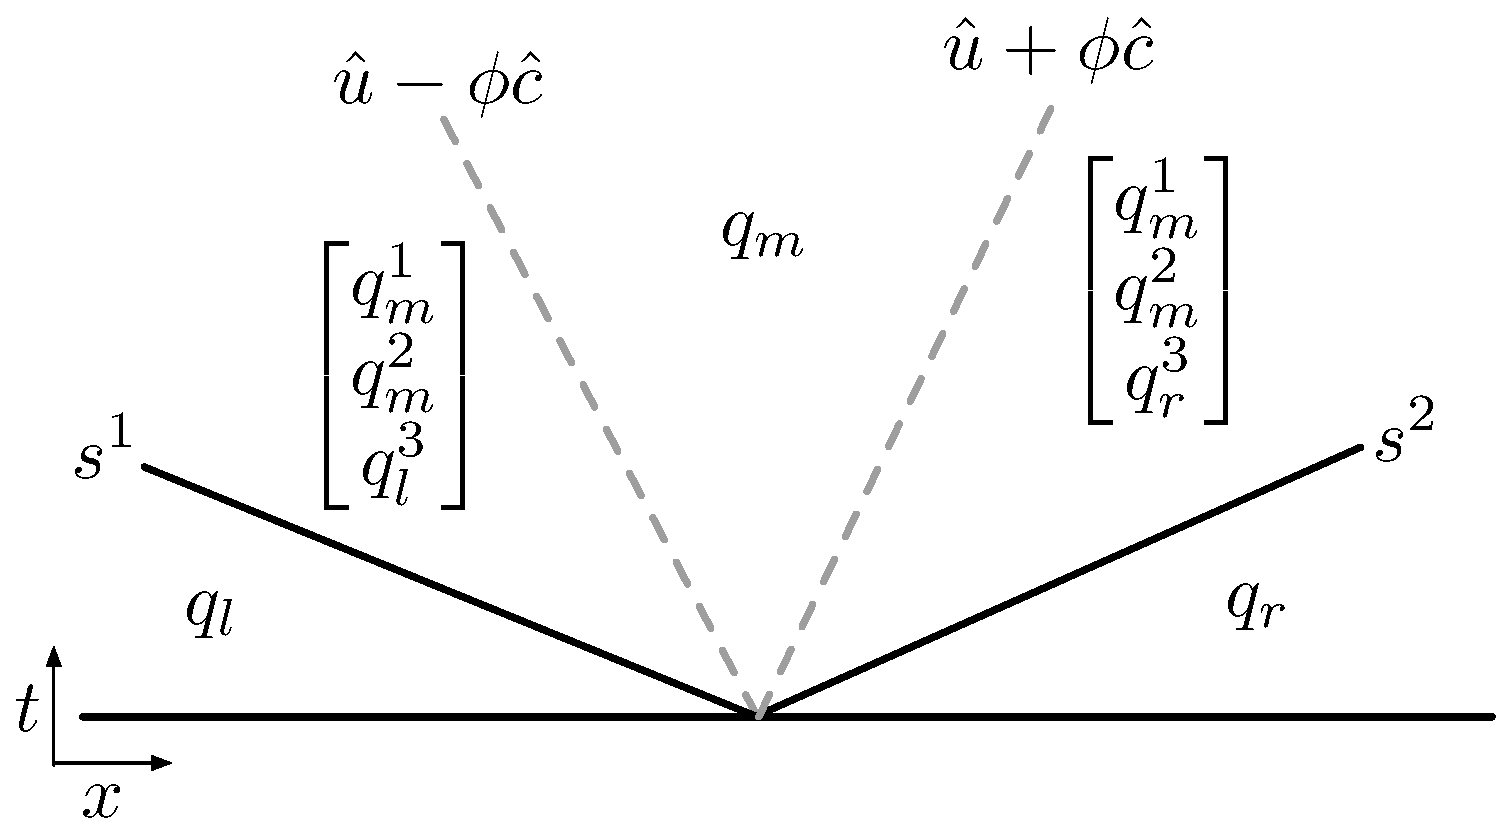
\includegraphics[width=0.6\textwidth]{figures/hllemcc.pdf}
%    \caption{Structure of the HLLEMCC approximate Riemann solution, with four waves.}
%    \label{HLLEMCC}
%\end{figure}

\subsection{The entropy residual}
Let $S_i$ be the set of cells containing cell $i$ and those that share a face with it.
Also let $\bfv(\bfu)=\eta^\prime(\bfu)$ be the entropy variable.
Based on \cite{guermond2011entropy}, we consider
\begin{align}\label{ent_residual}
  \int_{S_i} \bfv(\bfu) \cdot \left[ \frac{\partial \bfu}{\partial t} + \nabla\cdot \bff(\bfu)\right]d\bfx
  =\int_{S_i} \left[\frac{\partial \eta(\bfu)}{\partial t} + \bfv(\bfu) \cdot \nabla\cdot \bff(\bfu)\right] d\bfx
\end{align}
as a measurement of the entropy production in $S_i$.
To avoid the need to compute the time derivative of the entropy, we follow
\cite{guermond2018second, guermond2018well} and use
$\int \frac{\partial\eta(\bfu)}{\partial t}d\bfx=-\int \nabla\cdot\bfq(\bfu) d\bfx$,
which holds in smooth regions. Then we define
\begin{align}\label{Ri}
  \theta_i := \frac{R_i}{D_i},
\end{align}
with
\begin{align*}
  R_i=
  \left|\int_{S_i} \left[\bfv(\bfu) \cdot \nabla\cdot \bff(\bfu) - \nabla\cdot\bfq(\bfu) \right] d\bfx\right|,
\end{align*}
and $D_i$ being an upper bound of $R_i$ that acts as normalization so that $0\leq \theta_i\leq 1$.
Note that $R_i\approx 0$ if $\bfu$ is smooth in $S_i$.
In our implementation, we use
\begin{align*}
  R_i\approx \left|\bfv(\bfu_i)\cdot \int_{S_i}\nabla\cdot \bff(\bfu)d\bfx
  -\int_{S_i}\nabla\cdot\bfq(\bfu) d\bfx\right|,
  \quad
  %D_i = ||\bfv(\bfu_i)||_{\ell^2}\left|\left|\int_{S_i}\nabla\cdot\bff(\bfu)d\bfx\right|\right|_{\ell^2}
  %+\left|\int_{S_i}\nabla\cdot\bfq(\bfu)d\bfx\right|.
  D_i = \sum_{k=1}^{d+1}|\bfv_k(\bfu_i)|\left|\int_{S_i}\left(\nabla\cdot\bff(\bfu)\right)_kd\bfx\right|
  +\left|\int_{S_i}\nabla\cdot\bfq(\bfu)d\bfx\right|,
\end{align*}
where $({\bf z})_k$ denotes the $k$-th component of ${\bf z}\in\mathbb{R}^{d+1}$ and $d$ is the number of physical
dimensions. In the next section, we use $\theta_i$ to blend Rusanov's and Roe's Riemann solvers.

\subsection{Blended Riemann solver}\label{sec:blended_rs}
In this section, we use \eqref{Ri}, which is a normalized measurement of the entropy residual \eqref{ent_residual},
to blend Rusanov's and Roe's Riemann solvers. To do this, we define the blended numerical flux:
\begin{align}\label{num_flux_ev}
  F_{i+1/2} = \frac{\bff(\bfu_{i+1})+\bff(\bfu_i)}{2}
  - \frac{1}{2} \left( \theta_{i+1/2}\lambda_{i+1/2}^{\max} I + (1-\theta_{i+1/2})|\hat A_{i+1/2}| \right)(\bfu_{i+1}-\bfu_{i}).
\end{align}
Here $I\in\mathbb{R}^{3\times 3}$ is the identity matrix,
$\theta_{i+1/2}=\max\{\theta_{i+1},\theta_i\}$, $\lambda_{i+1/2}^{\max}$ is the
upper bound on the wave speed used in Rusanov's Riemann solver (see \S \ref{sec:rusanov}),
and $\hat A_{i+1/2}$ is Roe's averaged flux Jacobian (see \S \ref{sec:roe}).

The first-order method is given simply by \eqref{first-order_FV}
with the numerical flux $F_{i+1/2}$ given by \eqref{num_flux_ev}.
In smooth regions $\theta_{i+1/2}\approx 0$ so the numerical flux is essentially Roe's flux.
Near discontinuities or steep gradients, $\theta_{i+1/2}$ becomes large. In the limit $\theta_{i+1/2}\approx 1$
the numerical flux is essentially Rusanov's flux.

The first-order method can also be written in terms of fluctuations via \eqref{first-order_via_fluct}.
To do this we consider the waves ($\W^p_{i\pm 1/2}$, with $p=1,2,3$)
from Roe's solver and define
\begin{align}\label{lambda_p}
  \lambda_{i+1/2}^p := \theta_{i+1/2}\lambda_{i+1/2}^{\max} + (1-\theta_{i+1/2})|\hat \lambda_{i+1/2}^p|,
\end{align}
where $\hat\lambda_{i+1/2}^p$ is the $p$-th eigenvalue of Roe's solver corresponding to the
interface $i+1/2$. Note that $\lambda_{i+1/2}^p\geq 0$.
The fluctuations are then given by
\begin{subequations}\label{ev_fluctuations}
\begin{align}
  \apdq_\imh & = \frac{1}{2}\sum_p \left(\hat\lambda_{i-1/2}^p + \lambda_{i-1/2}^p\right)\W_{i-1/2}^p, \\
  \amdq_\iph & = \frac{1}{2}\sum_p \left(\hat\lambda_{i+1/2}^p - \lambda_{i+1/2}^p\right)\W_{i+1/2}^p.
\end{align}
\end{subequations}

To implement a second-order LWL scheme based on this solver, in addition to
these fluctuations we must define a set of waves and corresponding speeds.
Using only the waves from the Roe solver, it is in general not possible
to choose speeds that yield the fluctuations \eqref{ev_fluctuations}.
%In the framework of LeVeque, for a given interface $i+1/2$,
%we would need to consider a wave speed $s_{i+1/2}^p$ so that
%\begin{align*}
%  \hat \lambda_{i+1/2}^p+\lambda_{i+1/2}^p = s_{i+1/2}^p+|s_{i+1/2}^p|, \qquad
%  \hat \lambda_{i+1/2}^p-\lambda_{i+1/2}^p = s_{i+1/2}^p-|s_{i+1/2}^p|,
%\end{align*}
%which is not possible to obtain in general (since the problem is overdetermined).
Instead, we consider
$s_{i+1/2}^p=\sgn(\hat\lambda_{i+1/2}^p)\lambda_{i+1/2}^p$
 and study the consequences of this choice once the second-order corrections are applied.
Here $\sgn(z)$ is the sign function of $z$.
The second-order LWL method for the one-dimensional problem is given by
\begin{align}\label{second-order}
  u_i^{n+1}=u_i^n
  -\frac{\Delta t}{\Delta x}\left[\A^-\Delta Q_{i+1/2}+\A^+\Delta Q_{i-1/2}\right]
  -\frac{\Delta t}{\Delta x}\left[\tilde F_{i+1/2}-\tilde F_{i-1/2}\right],
\end{align}
where
\begin{align*}
  \tilde F_{i+1/2} = \frac{1}{2}\sum_p\lambda_{i+1/2}^p
  \left(1-\frac{\Delta t}{\Delta x}\lambda_{i+1/2}^p\right)\tilde\W_{i+1/2}^p
\end{align*}
are the flux corrections with $\tilde\W_{i+1/2}^p$ being a limited version of $\W_{i+1/2}^p$.

To understand the effect of choosing $s_{i+1/2}^p=\sgn(\hat\lambda_{i+1/2}^p)\lambda_{i+1/2}^p$
as the speed of $\W_{i+1/2}^p$,
let us assume that no limiters are applied; i.e., $\tilde\W_{i\pm 1/2}^p\equiv \W_{i\pm 1/2}^p$.
By doing this, equation \eqref{second-order} can be written as
\begin{align*}
  u_i^{n+1}=u_i^n
  &-\frac{\Delta t}{2 \Delta x}
  \sum_p
  \left[\left(\hat\lambda_{i+1/2}^p -\frac{\Delta t}{\Delta x}(\lambda_{i+1/2}^p)^2 \right)\W_{i+1/2}^p
  +
  \left(\hat\lambda_{i-1/2}^p +\frac{\Delta t}{\Delta x}(\lambda_{i-1/2}^p)^2 \right)\W_{i-1/2}^p\right],
\end{align*}
which corresponds to the standard Lax-Wendroff method written in terms of fluctuation-like quantities.
Note that if $\theta_{i\pm 1/2}=0$, we recover the standard second-order Lax-Wendroff method based on
Roe's Riemann solver.
In the numerical experiments in \S\ref{sec:num}, we obtain second-order experimental
order of convergence (EOC) for problems with smooth solution, which is expected since
$\theta_{i\pm 1/2}\approx 0$ in smooth regions.
Similarly, if $\theta_{i\pm 1/2}=1$, we recover the Lax-Wendroff method based on Rusanov's Riemann solver,
which can be seen by writing the fluctuations in Rusanov's method in terms of Roe's waves and speeds.

To see this, first consider \eqref{rus_cons} and rewrite the right-going fluctuation as follows:
\begin{align}\label{rus_rs_aux}
  \A^{+,\Rus}\Delta Q_{i-1/2}:=\lambda_{i-1/2}^{\max}\W_{i-1/2}^{2,\max}
  = \bff(\bfu_{i})-\bff(\bfu_{i-1}) + \lambda_{i-1/2}^{\max}\left(\W_{i-1/2}^{1,\Rus}+\W_{i-1/2}^{2,\Rus}\right)
  -\lambda_{i-1/2}^{\max}\W_{i-1/2}^{2,\Rus}.
  %\A^{+,\Rus}\Delta Q_{i-1/2}=\frac{1}{2}\sum_p\left(\hat \lambda_{i-1/2}^p + \lambda_{i-1/2}^{\max}\right)\W_{i-1/2}^p
\end{align}
From \eqref{system_for_alphas} and \eqref{rusanov_waves} we get
$\W^{1,\Rus}_{i-1/2}+\W^{2,\Rus}_{i-1/2}=\bfu_i-\bfu_{i-1}=\sum_p\W_{i-1/2}^p$.
Using \eqref{rs_conservation}, \eqref{rus_rs_aux} becomes
\begin{align*}
  \lambda_{i-1/2}^{\max}\W_{i-1/2}^{2,\max}
  = \sum_p \left(\hat \lambda_{i-1/2}^p + \lambda_{i-1/2}^{\max}\right)\W_{i-1/2}^p
  -\lambda_{i-1/2}^{\max}\W_{i-1/2}^{2,\Rus},
\end{align*}
which implies that
\begin{subequations}\label{fluct_rus}
\begin{align}
  \A^{+,\Rus}\Delta Q_{i-1/2}=\frac{1}{2}\sum_p\left(\hat \lambda_{i-1/2}^p + \lambda_{i-1/2}^{\max}\right)\W_{i-1/2}^p,
\end{align}
and similarly,
\begin{align}
  \A^{-,\Rus}\Delta Q_{i+1/2}=\frac{1}{2}\sum_p\left(\hat \lambda_{i+1/2}^p - \lambda_{i+1/2}^{\max}\right)\W_{i+1/2}^p.
\end{align}
\end{subequations}


\subsection{Entropy-stable Riemann solver}\label{sec:entropy_stable}
The Riemann solver presented in the previous section blends the solvers of Rusanov and Roe based on a
local measurement of the entropy residual. The objective is to induce dissipation of entropy
near discontinuities. However, we have no guarantee that methods \eqref{first-order_via_fluct}
or \eqref{second-order_via_fluct} based on this Riemann solver are (locally) entropy stable.
In this section, we further modify the first-order method
\eqref{first-order_via_fluct} in order to guarantee local entropy stability.

Let $\bfv_i=\bfv(\bfu_i)$ and $q_i=q(\bfu_i)$ denote the entropy variable and the
(one-dimensional) entropy potential at cell $i$, respectively.
Also let $\psi_i=\bfv(\bfu_i)\cdot \bff(\bfu_i)-q(\bfu_i)$ be the entropy potential at cell $i$.
From \cite[\S 4]{tadmor1987numerical}, if the numerical fluxes satisfy
\begin{align}\label{es_cond}
(\bfv_{i}-\bfv_{i-1})\cdot \bfF_{i-1/2}\leq \psi_{i}-\psi_{i-1},
  \qquad
  (\bfv_{i+1}-\bfv_i)\cdot \bfF_{i+1/2}\leq \psi_{i+1}-\psi_i,
\end{align}
then the following entropy inequality holds
\begin{align}\label{ent_ineq}
  \frac{d\eta(\bfu_i)}{dt}+\frac{1}{\Delta x}\left[G_{i+1/2}-G_{i-1/2}\right]\leq 0,
\end{align}
where
\begin{align*}
    G_{i+1/2} &= \frac{1}{2}\left(\bfv_i+\bfv_{i+1}\right)\bfF_{i+1/2}-\frac{1}{2}(\psi_{i}+\psi_{i+1}),
\end{align*}
is the discrete entropy flux.

To enforce \eqref{es_cond} we further modify the flux \eqref{num_flux_ev}:
\begin{align*}
  \bfF_{i+1/2} = \frac{\bff(\bfu_{i+1})+\bff(\bfu_i)}{2}
  - \frac{1}{2} \left( \theta_{i+1/2}\lambda_{i+1/2}^{\max}\mathbb{I} + (1-\theta_{i+1/2})|\hat A_{i+1/2}| +\lambda_{i+1/2}^{\min}\mathbb{I}\right)(\bfu_{i+1}-\bfu_{i}).
\end{align*}
Here $\lambda_{i+1/2}^{\min}$ is yet to be defined.
We can write the numerical fluxes in terms of $\lambda^p_{i\pm 1/2}$ \eqref{lambda_p}
and Roe's waves $\W_{i\pm 1/2}^p$.
Doing so, we get
\begin{align*}
  \bfF_{i+1/2} = \frac{\bff(\bfu_{i+1})+\bff(\bfu_i)}{2}
  - \frac{1}{2}\sum_p(\lambda_{i+1/2}^p+\lambda_{i+1/2}^{\min})\W_{i+1/2}^p.
\end{align*}

We set
\begin{align}\label{lambda_min}
  \lambda_{i+1/2}^{\min} = \max\left\{0,\frac{\frac{1}{2}(\bfv_{i+1}-\bfv_{i})\cdot\left[\bff(\bfu_{i+1})+\bff(\bfu_{i})-\sum_p\lambda_{i+1/2}^p\W_{i+1/2}^p\right]-(\psi_{i+1}-\psi_i)}{\frac{1}{2}(\bfv_{i+1}-\bfv_{i})\cdot\sum_p\W_{i+1/2}^p}\right\}
\end{align}
which guarantees \eqref{es_cond}, and therefore \eqref{ent_ineq}.

Since the blended Riemann solver described in Section \ref{sec:blended_rs} already
tends to introduce entropy dissipation,
we expect condition \eqref{es_cond} to be fulfilled most of the time even with $\lambda_{i+1/2}^{\min}=0$.
But \eqref{lambda_min} is used as a safeguard to guarantee entropy stability of the first-order method.
Extra modifications would be needed to guarantee entropy stability of the second-order LWL method
\eqref{second-order_via_fluct} and its multidimensional extension via Strang splitting.
We do not pursue such modifications in this work.

\begin{remark}
In terms of fluctuations, the entropy stability condition \eqref{es_cond} can be written as
\begin{align*}
  (\bfv_{i}-\bfv_{i-1})\cdot
  \Big(
  \underbrace{\bff(\bfu_i)-\A^+\Delta Q_{i-1/2}}_{=\bfF_{i-1/2}}\Big)\leq \psi_{i}-\psi_{i-1},
  \quad
  (\bfv_{i+1}-\bfv_i)\cdot
  \Big(\underbrace{\bff(\bfu_i)+\A^-\Delta Q_{i+1/2}}_{=\bfF_{i+1/2}}\Big)\leq \psi_{i+1}-\psi_i.
\end{align*}
\end{remark}

\begin{remark}[About the effect of $\lambda_{i\pm 1/2}^{\min}$ for Roe's solver.]
  If we set $\theta_{i\pm 1/2}=0, ~\forall i$ in \eqref{lambda_p}, then the Riemann solver becomes Roe's solver.
  In this case, it is well known that transonic rarefactions develop non-physical shocks,
  a phenomenon known as `entropy glitch'. To fix this problem, many entropy fixes to Roe's
  solver have been developed. Enhancing the dissipation via \eqref{lambda_min}
  also serves as a transonic entropy fix for Roe's solver, which we demonstrate
  via a numerical experiment in \S \ref{sec:rp_dry_bed}.
\end{remark}

\clearpage
\section{Numerical results}\label{sec:num}
In this section we present one- and two-dimensional numerical experiments to demonstrate the behavior of the
blended Riemann solver from \S\ref{sec:blended_rs} with the extra entropy dissipation from \S\ref{sec:entropy_stable}.
We compare the behavior of the blended solver against the standard Roe's and Rusanov's solvers.
In most of the experiments we use these Riemann solvers with the LWL method reviewed in \S\ref{sec:waveprop}.
When the exact solution is available, we report a convergence test based on the $L^1$-error for the water height
\begin{align*}
  E_1=\sum_i|K_i|~|h_i-h^e(\bfx_i)|,
\end{align*}
where $|K_i|$ is the length or area of cell $i$,
$h_i$ is the cell average of the water height at cell $i$,
and $h^e(\bfx_i)$ is the exact water height evaluated at the center of cell $i$.

We consider a total of six problems. We start with a one-dimensional Riemann problem over a dry bed.
For this problem we use the first-order method \eqref{first-order_via_fluct},
which helps preventing violations of positivity. Although, only Rusanov's solver guarantees
positivity, we do not get negative values for the water height with this method and the other Riemann solvers.
In \S \ref{sec:steady_outflow} we consider a one-dimensional problem with a smooth steady state solution. We observe the expected
second-order accuracy of method \eqref{second-order_via_fluct} with Roe's and the blended solvers. Using
Rusanov's Riemann solver degrades the accuracy to first-order. The overall accuracy of the blended solver
is not degraded since the extra dissipation is not applied in smooth regions.
In \S\ref{sec:rp_wet_bed} and \S\ref{sec:1D_chj} we consider one-dimensional problems with strong shocks. We observe similar accuracy with the
blended solver than with Roe's solver; that is, inducing entropy dissipation near the shocks do not degrade the accuracy
of the underlying Roe's solver. This extra dissipation, however, prevents the formation of carbuncles in other experiments,
which we demonstrate in \S \ref{sec:bow_shock} and \S\ref{sec:2D_chj}.
The main focus of this work is in the formation of carbuncle instabilities in the two-dimensional CHJ. We present
an extensive set of experiments about this problem in \S \ref{sec:2D_chj}.
We consider not only Roe's, Rusanov's and the blended solvers, but also the HLLE solver and a solver proposed in \cite{kemm2014note},
which is designed to remove the carbuncle instabilities in the shallow water equations.

\subsection{Dam break problem on a dry bed}\label{sec:rp_dry_bed}
We start with the one-dimensional dam break problem on a dry bed.
This problem is a canonical example that demonstrates the `entropy glitch' of Roe's solver
at transonic rarefactions. Since the baseline Roe's solver we use (see \S\ref{sec:roe}) does not contain
an entropy fix, it is important to demonstrate that the blended Riemann solver fixes the entropy glitch.
We follow the setup in \cite[\S 4.1.2]{delestre2013swashes}.
The domain is given by $\Omega=(0,L=10)$, and the initial condition is $hu(x,0)=0$ and
\begin{align*}
  h(x,0)=
  \begin{cases}
    h_l, & \mbox{ if }, x\leq x_0=5 \\
    h_r, &\mbox{ otherwise},
  \end{cases}
\end{align*}
with $h_l=5\times 10^{-3}$ and $h_r=0$. In our experiments we use $h_r=1\times 10^{-15}$ to avoid division by zero.
The exact solution, which can also be found in \cite{delestre2013swashes} and references therein, is
\begin{align*}
  h(x,t) =
  \begin{cases}
    h_l, \\
    \frac{4}{9g}\left(\sqrt{gh_l}-\frac{x-x_0}{2t}\right)^2, \\
    0,
  \end{cases}
\quad
  u(x,t) =
  \begin{cases}
    0, &\mbox{ if } x\leq x_A(t), \\
    \frac{2}{3}\left(\sqrt{gh_l}+\frac{x-x_0}{t}\right), & \mbox{ if } x_A(t) < x\leq x_B(t), \\
    0, &\mbox{ if } x_B(t)\leq x,
  \end{cases}
\end{align*}
with $x_A(t)=x_0-t\sqrt{gh_l}$ and $x_B(t)=x_0+2t\sqrt{gh_l}$.
We use $g=1$ and solve the problem up to $t=10$.
In figures \ref{fig:rp_dry_bed_roe}-\ref{fig:rp_dry_bed_blended},
we show the solution using method \eqref{first-order_via_fluct}
with Roe's solver, Rusanov's solver and the blended solver, respectively.
The entropy glitch, which is manifested as a non-physical shock at $x=x_0$,
is present with Roe's solver. Using Rusanov's and the blended solvers
fixes the entropy glitch.
In Table \ref{table:rp_dry_bed}, we summarize the results of a convergence test.
Note that using the blended solver leads to more accurate results.

\begin{figure}[!h]
  {\scriptsize
    \subfloat[Roe's Riemann solver.\label{fig:rp_dry_bed_roe}]{
      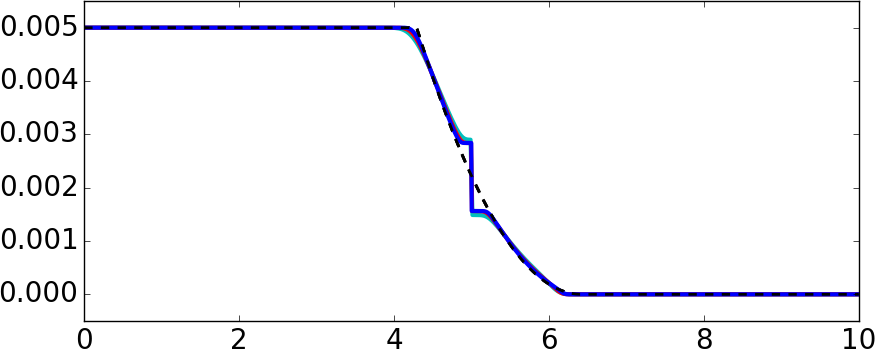
\includegraphics[scale=0.36]{figures/rp_dry_roe.png}}
    ~
    \subfloat[Rusanov's Riemann solver.\label{fig:rp_dry_bed_llf}]{
        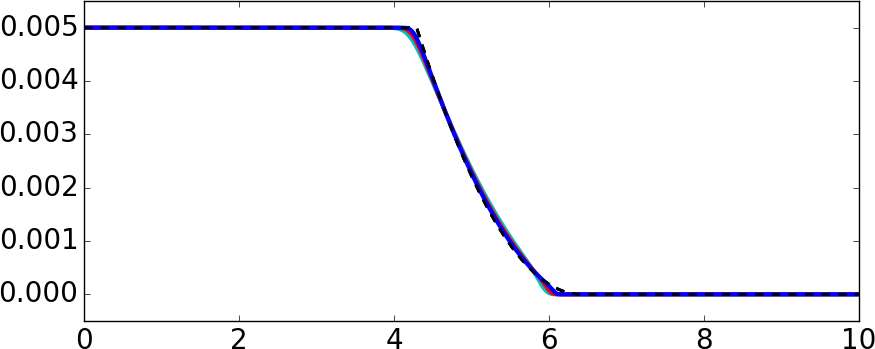
\includegraphics[scale=0.36]{figures/rp_dry_llf.png}}

    \subfloat[Blended Riemann solver. \label{fig:rp_dry_bed_blended}]{
      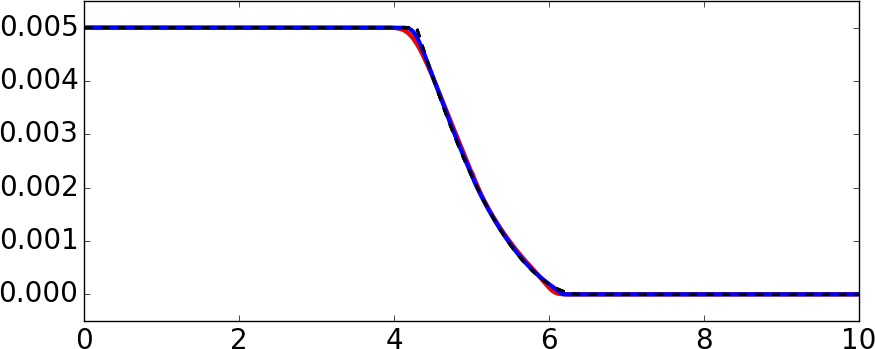
\includegraphics[scale=0.36]{figures/rp_dry_blended.png}}
    ~
    \subfloat[Roe's Riemann solver with $\lambda_{i\pm 1/2}^{\min}$.\label{fig:rp_dry_bed_roe_with_lmin}]{
      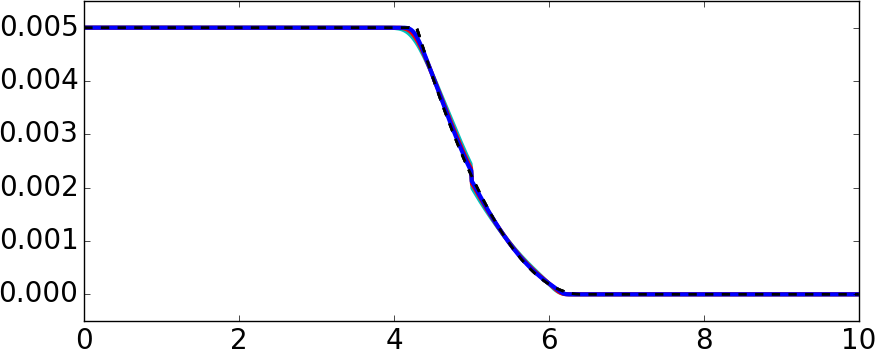
\includegraphics[scale=0.36]{figures/rp_dry_roe_with_lmin.png}}
  }
  \caption{
    Dam break problem over a dry bed using method \eqref{first-order_via_fluct} with different
    Riemann solvers. We show the numerical solution and the exact solution (in dashed black) at $t=10$.
    We consider different refinements with
    (cyan) $\Delta x=1/400$, (red) $\Delta x=1/800$, (blue) $\Delta x=1/1600$.
    \label{fig:rp_dry_bed}}
\end{figure}

For this particular problem, using method \eqref{first-order_via_fluct} with the blended Riemann solver
leads to $\lambda_{i\pm 1/2}^{\min}=0$ for all the experiments, but this is not true in general.
Finally, let us demonstrate the effect of $\lambda_{i\pm 1/2}^{\min}$ by imposing $\theta_{i}=0$ in \eqref{lambda_p},
which is equivalent to using Roe's solver with extra dissipation given by $\lambda_{i\pm 1/2}^{\min}$.
In Figure \ref{fig:rp_dry_bed_roe_with_lmin}, we show the solution using different refinements,
and in the last column of Table \ref{table:rp_dry_bed}, we summarize the results of a convergence test.
Note that the entropy glitch is highly reduced.
To remove completely the entropy glitch we could add high-order entropy dissipation following \cite{tadmor2003entropy}
and references therein.

\begin{table}[!ht]\scriptsize
  \begin{center}
    \begin{tabular}{||c||c|c||c|c||c|c||c|c||} \hline
      & \multicolumn{2}{c||}{Roe's solver}
      &\multicolumn{2}{c||}{Rusanov's solver}
      &\multicolumn{2}{c||}{Blended solver}
      &\multicolumn{2}{c||}{Roe's with $\lambda_{i\pm 1/2}^{\min}$} \\ \cline{2-9}
      $\Delta x$ & $E_1$ & rate & $E_1$ & rate & $E_1$ & rate & $E_1$ & rate \\ \hline
      1/50   & 6.21E-04 &  --  & 6.95E-04 &   -- & 5.10E-04 &  --  & 5.95E-04 & --   \\
      1/100  & 4.70E-04 & 0.40 & 5.27E-04 & 0.40 & 3.53E-04 & 0.52 & 4.06E-04 & 0.55 \\
      1/200  & 3.91E-04 & 0.26 & 3.88E-04 & 0.44 & 2.38E-04 & 0.56 & 2.83E-04 & 0.52 \\
      1/400  & 3.16E-04 & 0.30 & 2.64E-04 & 0.55 & 1.51E-04 & 0.65 & 1.89E-04 & 0.58 \\
      1/800  & 2.35E-04 & 0.42 & 1.67E-04 & 0.66 & 9.43E-05 & 0.68 & 1.20E-04 & 0.65 \\
      1/1600 & 2.00E-04 & 0.23 & 1.01E-04 & 0.72 & 5.70E-05 & 0.72 & 7.42E-05 & 0.68 \\ \hline
    \end{tabular}
    \caption{Grid convergence study for the dam break problem over a dry bed
      using method \eqref{first-order_via_fluct} with different Riemann solvers.\label{table:rp_dry_bed}}
  \end{center}
\end{table}

\subsection{Dam break problem on a wet bed}\label{sec:rp_wet_bed}
We consider now a one-dimensional dam break problem on a wet domain.
We follow the setup in \cite[\S 4.1.1]{delestre2013swashes}.
The domain is $\Omega=(0,L)$ with $L=10$, the initial condition is given by
$hu(x,0)=0$ and
\begin{align*}
  h(x,0) =
  \begin{cases}
    h_l & \mbox{ if } x\in(0,x_0], \\
    h_r & \mbox{ if } x\in(x_0,L),
  \end{cases}
\end{align*}
with $x_0=5$, $h_l=0.005$ and $h_r=0.001$.
The exact solution, which can be found in \cite{delestre2013swashes} and references therein,
is given by
\begin{align*}
  h(x,t) =
  \begin{cases}
    h_l, \\
    \frac{4}{9g}\left(\sqrt{gh_l}-\frac{x-x_0}{2t}\right)^2, \\
    \frac{c_m^2}{g}, \\
    h_r,
  \end{cases}
\quad
  u(x,t) =
  \begin{cases}
    0, &\mbox{ if } x\leq x_A(t), \\
    \frac{2}{3}\left(\sqrt{gh_l}+\frac{x-x_0}{t}\right), & \mbox{ if } x_A(t) < x\leq x_B(t), \\
    2(\sqrt{gh_l}-c_m), & \mbox{ if } x_B(t)<x\leq x_C(t), \\
    0, &\mbox{ if } x\leq x_C(t),
  \end{cases}
\end{align*}
where $x_A(t)=x_0-t\sqrt{gh_l}$, $x_B(t)=x_0+t\left(2\sqrt{gh_l}-3c_m\right)$,
$x_C(t)=x_0+t\frac{2c_m^2\left(\sqrt{gh_l}-c_m\right)}{c_m^2-gh_r}$ and
$c_m$ is the solution of
$-8gh_rc_m^2\left(\sqrt{gh_l}-c_m\right)^2+\left(c_m^2-gh_r\right)^2\left(c_m^2+gh_r\right)=0$.
We use $g=1$ and solve the problem up to the final time $t=5$ considering method \eqref{second-order_via_fluct}
with Roe's, Rusanov's and the blended solvers. The solution with different refinement levels
and each Riemann solver is shown in Figure \ref{fig:rp_wet_bed}.
In Table \ref{table:rp_wet_bed}, we summarize the results of a convergence test.
Since the solution is non-smooth, we expect no more than first order convergence rates. Note that the
results with the entropy dissipative blended solver are comparable against the results using Roe's solver.
That is, inducing entropy dissipation via the blended Riemann solver does not degrade the high-order
accuracy properties of Roe's solver.
In contrast, the accuracy and convergence rates using Rusanov's solver are clearly degraded.

\begin{figure}[!h]
  {\scriptsize
    \subfloat[Roe's Riemann solver.]{
      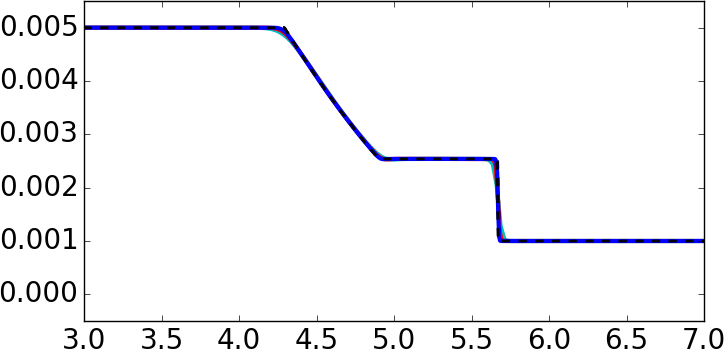
\includegraphics[scale=0.29]{figures/rp_wet_roe.png}}
    \quad
    \subfloat[Rusanov's Riemann solver.]{
        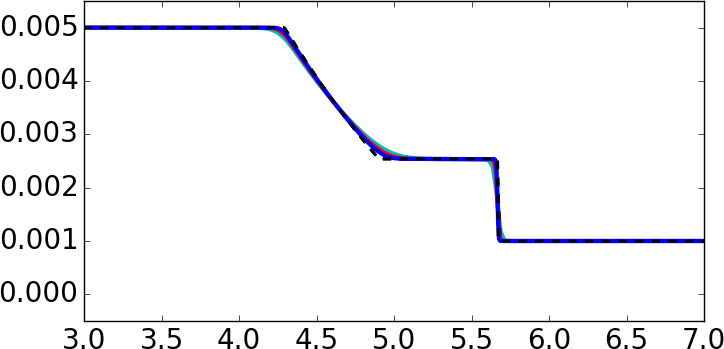
\includegraphics[scale=0.29]{figures/rp_wet_llf.png}}
    \quad
    \subfloat[Blended Riemann solver.]{
      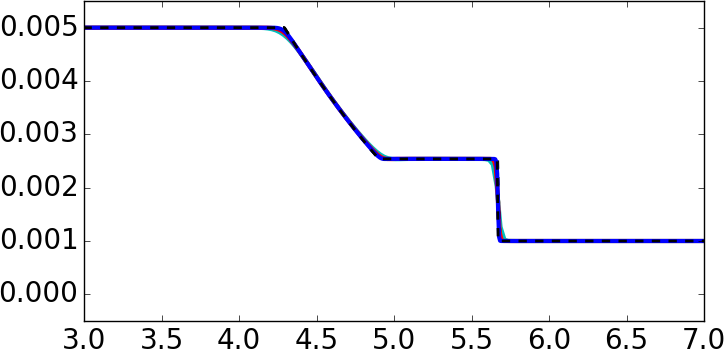
\includegraphics[scale=0.29]{figures/rp_wet_blended.png}}
  }
  \caption{
    Dam break problem over a wet bed using method \eqref{second-order_via_fluct} with different
    Riemann solvers. We show the numerical solution and the exact solution (in dashed black) at $t=10$.
    We consider different refinements with
    (cyan) $\Delta x=1/400$, (red) $\Delta x=1/800$, (blue) $\Delta x=1/1600$.
    \label{fig:rp_wet_bed}}
\end{figure}

\begin{table}[!ht]\scriptsize
  \begin{center}
    \begin{tabular}{||c||c|c||c|c||c|c||} \hline
      & \multicolumn{2}{c||}{Roe's solver}
      &\multicolumn{2}{c||}{Rusanov's solver}
      &\multicolumn{2}{c||}{Blended solver} \\ \cline{2-7}
      $\Delta x$ & $E_1$ & rate & $E_1$ & rate & $E_1$ & rate \\ \hline
      1/50   & 4.22E-04 &  --  & 5.73E-04 &  --  & 4.34E-04 & --   \\
      1/100  & 2.00E-04 & 1.07 & 3.35E-04 & 0.78 & 2.08E-04 & 1.05 \\
      1/200  & 1.11E-04 & 0.85 & 2.01E-04 & 0.74 & 1.13E-04 & 0.88 \\
      1/400  & 5.05E-05 & 1.13 & 1.18E-04 & 0.77 & 5.26E-05 & 1.10 \\
      1/800  & 2.60E-05 & 0.95 & 7.08E-05 & 0.74 & 2.73E-05 & 0.94 \\
      1/1600 & 1.29E-05 & 1.01 & 3.79E-05 & 0.90 & 1.32E-05 & 1.04 \\ \hline
    \end{tabular}
    \caption{Grid convergence study for the dam break problem over a wet bed
      using method \eqref{second-order_via_fluct} with different Riemann solvers.\label{table:rp_wet_bed}}
  \end{center}
\end{table}

\subsection{The circular hydraulic jump in one-dimension}\label{sec:1D_chj}
In this section we consider for the first time a CHJ. We start with a one-dimensional problem
embedded into the two-dimensional domain $\Omega=(0.1,1)\times(0,0.1)$.
A semi-analytical solution at steady state is available as described in \S \ref{sec:steady_chj};
therefore, we can perform a convergence test.
We consider the initial condition $h(x,t=0)=0.1$, $hu(x,t=0)=0$ and $hv(x,t=0)=0$.
At the left boundary, we impose $h(0.1,t)=0.3$, $hu(0.1,t)=0.225$ and $hv(0.1,t)=0$.
At the right boundary we impose $h(1,t)=0.37387387318873766$, $hu(1,t)=\beta/h(1,t)$ and $hv(1,t)=0$ where $\beta=0.0225$.
The values on the right boundary are chosen so that the CHJ is located at $x=0.3$, as described in \S \ref{sec:formation}.
%
In the first row of Figure \ref{fig:rp_wet_bed}, we show (slices of) the solution (at $y=0.05$)
at different times using the second-order method \eqref{second-order_via_fluct} with Roe's, Rusanov's and the blended Riemann solvers.
In the second row of the same figure, we plot $\theta_i$ \eqref{Ri}, which is a (normalized) measurement of the
entropy residual. Note that $\theta_i$ accurately locates the shocks and is (nearly) zero in smooth regions.
In Table \ref{table:chj_1D}, we summarize the results of a convergence study.
We remark that the convergence with Roe's solver is erratic.
Moreover, for the finer grids, the solution appears to become worse.
Using Rusanov's and the blended Riemann solvers delivers cleaner convergence rates.
In \cite[\S 5]{kemm2018heuristical} and \cite{bader2014carbuncle}, the authors consider one-dimensional problems embedded into
two-dimensional domains and observe different instabilities for the
Euler and the shallow water equations, respectively.
The authors attributed the problem to a manifestation of the carbuncle instability
that lead to an unstable location of the steady shock with certain Riemann solvers, including Roe's solver.

\begin{figure}[!h]
  {\scriptsize
    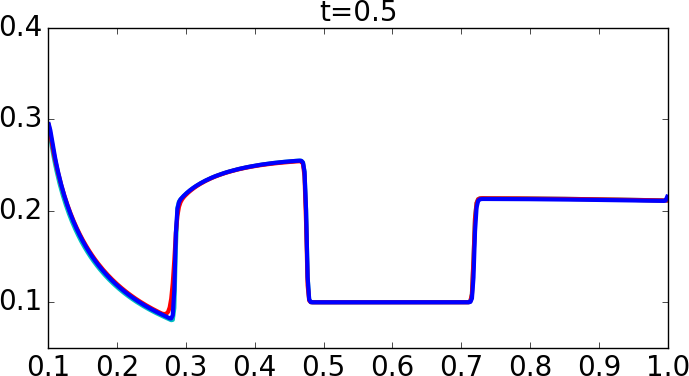
\includegraphics[scale=0.29]{figures/chj_1D_t0p5.png}
    \qquad
    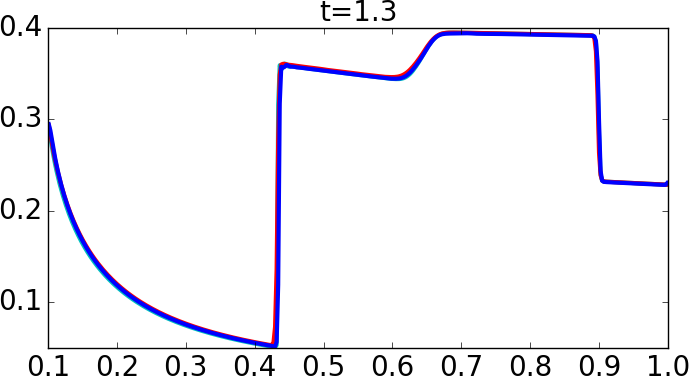
\includegraphics[scale=0.29]{figures/chj_1D_t1p3.png}
    \qquad
    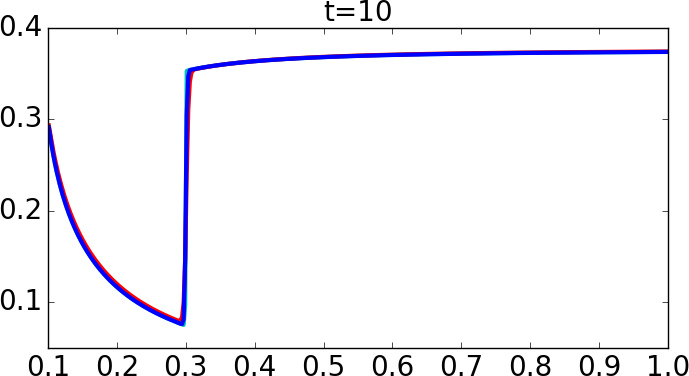
\includegraphics[scale=0.29]{figures/chj_1D_t10p0.png}

    \vspace{15pt}
    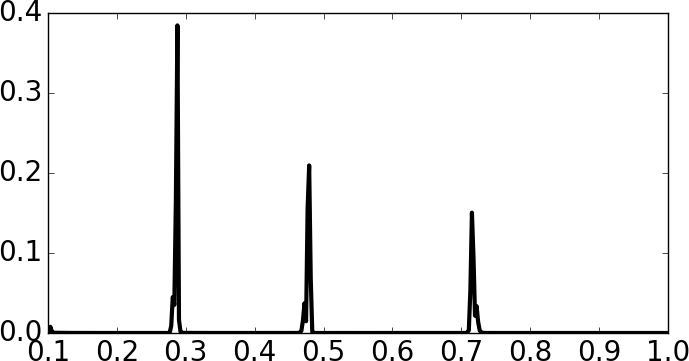
\includegraphics[scale=0.29]{figures/chj_1D_Ri_t0p5.png}
    \qquad
    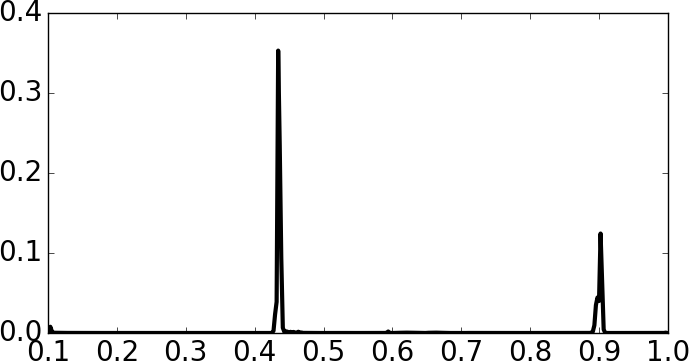
\includegraphics[scale=0.29]{figures/chj_1D_Ri_t1p3.png}
    \qquad
    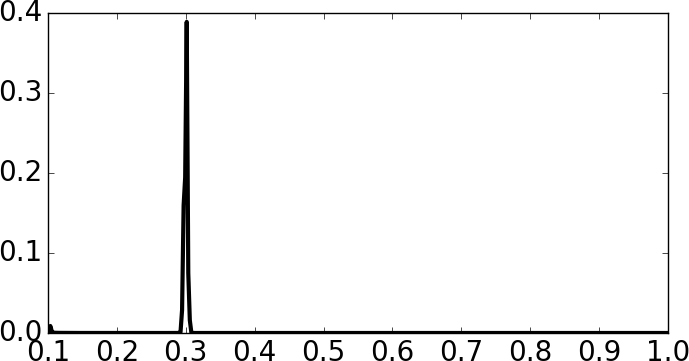
\includegraphics[scale=0.29]{figures/chj_1D_Ri_t10p0.png}
  }
  \caption{
    One-dimensional CHJ using method \eqref{second-order_via_fluct} with
    (cyan) Roe's, (red) Rusanov's and (blue) the blended Riemann solvers.
    In the second row we plot $\theta_i$, which is given by \eqref{Ri}.
    In all simulations we consider $\Delta x=1/400$.
    \label{fig:1D_chj}}
\end{figure}

\begin{table}[!ht]\scriptsize
  \begin{center}
    \begin{tabular}{||c||c|c||c|c||c|c||} \hline
      & \multicolumn{2}{c||}{Roe's solver}
      &\multicolumn{2}{c||}{Rusanov's solver}
      &\multicolumn{2}{c||}{Blended solver} \\ \cline{2-7}
      $\Delta x$ & $E_1$ & rate & $E_1$ & rate & $E_1$ & rate \\ \hline
      1/50  & 1.56E-04 &  --   & 8.80E-04 &  --  & 3.56E-04 &  --  \\
      1/100 & 1.06E-04 & 0.55  & 5.09E-04 & 0.79 & 1.95E-04 & 0.86 \\
      1/200 & 7.77E-05 & 0.45  & 2.96E-04 & 0.78 & 1.07E-04 & 0.87 \\
      1/400 & 7.50E-06 & 3.37  & 1.49E-04 & 0.99 & 3.68E-05 & 1.53 \\
      1/800 & 9.07E-06 & -0.27 & 7.98E-05 & 0.90 & 1.67E-05 & 1.14 \\ \hline
    \end{tabular}
    \caption{Grid convergence study for the one-dimensional CHJ at $t=10$
      using method \eqref{second-order_via_fluct} with different Riemann solvers.\label{table:chj_1D}}
  \end{center}
\end{table}

\subsection{Steady outflow}\label{sec:steady_outflow}
Let us consider a problem similar to that in the previous section, but with an outflow boundary condition.
That is, we consider the one-dimensional domain $\Omega=(0.1,1)$, the initial condition
$h(x,t=0)=0.1$, $hu(x,t=0)=0$, the left boundary condition $h(0.1,t)=0.3$, $hu(0.1,t)=0.75$,
and set the right boundary condition to outflow.
We refer to \cite[\S 21.8.5]{leveque2002finite} for details about the outflow boundary condition.
If the flow is supercritical ($|F|>1$ where $F$ is the Froude number), the exact solution converges to a
steady state profile given by the solution of \eqref{steady}.
Depending on the initial condition, shocks might develop before the steady state is reached.
Nevertheless, the steady state profile is smooth.
In Figure \ref{fig:steady_outflow}, we show the solution and $\theta_i$ at different times using
the second-order method \eqref{second-order_via_fluct}
with Roe's, Rusanov's and the blended Riemann solvers.
Additionally, in Table \ref{table:steady_outflow}, we summarize the results of a convergence study
based on methods \eqref{first-order_via_fluct} and
\eqref{second-order_via_fluct}, using the same Riemann solvers.

\begin{figure}[!h]
  {\scriptsize
    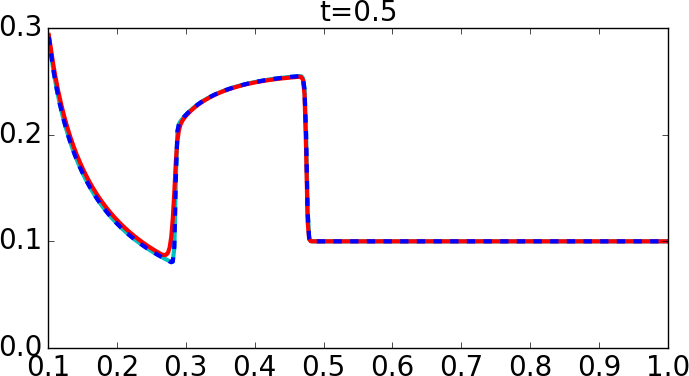
\includegraphics[scale=0.29]{figures/outflow_1D_t0p5.png}
    \qquad
    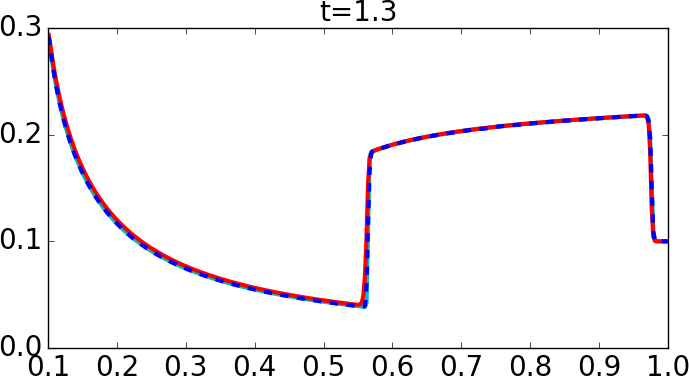
\includegraphics[scale=0.29]{figures/outflow_1D_t1p3.png}
    \qquad
    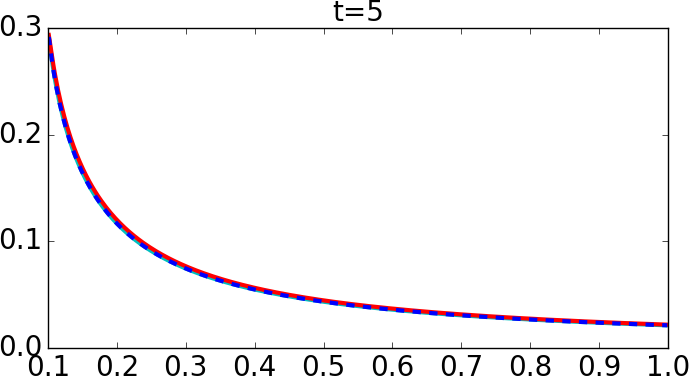
\includegraphics[scale=0.29]{figures/outflow_1D_t10p0.png}

    \vspace{15pt}
    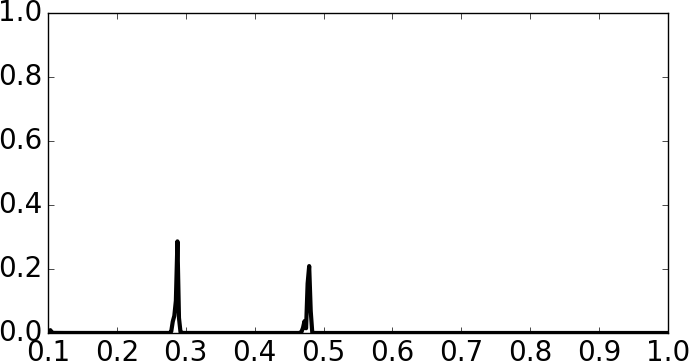
\includegraphics[scale=0.29]{figures/outflow_1D_Ri_t0p5.png}
    \qquad
    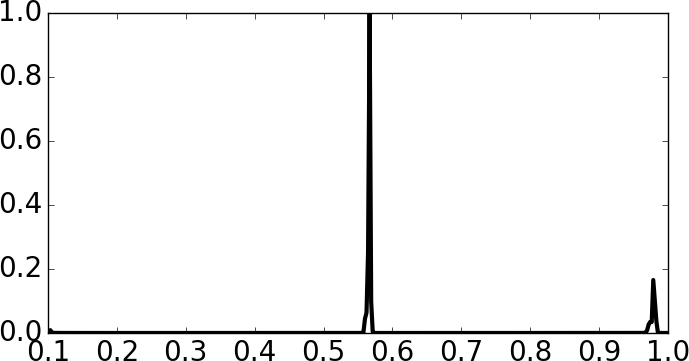
\includegraphics[scale=0.29]{figures/outflow_1D_Ri_t1p3.png}
    \qquad
    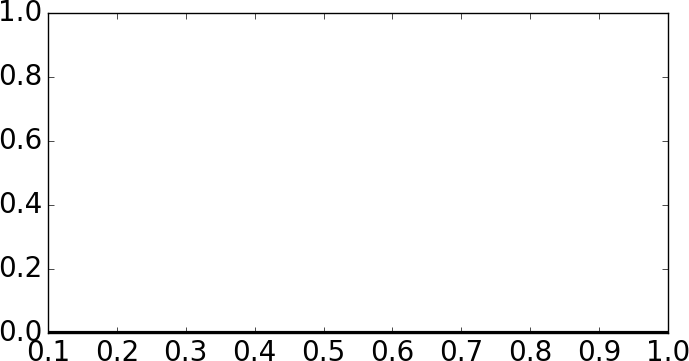
\includegraphics[scale=0.29]{figures/outflow_1D_Ri_t10p0.png}
  }
  \caption{
    Steady outflow problem using method \eqref{second-order_via_fluct} with
    (cyan) Roe's, (red) Rusanov's and (dashed blue) the blended Riemann solvers.
    In the second row we plot $\theta_i$, which is given by \eqref{Ri}.
    In all simulations we consider $\Delta x=1/400$.
    \label{fig:steady_outflow}}
\end{figure}

\begin{table}[!ht]\scriptsize
  \begin{center}
    \begin{tabular}{||c||c|c||c|c||c|c||c|c||c|c||c|c||} \hline
      & \multicolumn{6}{c||}{First-order method \eqref{first-order_via_fluct}}
      & \multicolumn{6}{c||}{Second-order method \eqref{second-order_via_fluct}} \\ \cline{2-13}
      & \multicolumn{2}{c||}{Roe's solver}
      &\multicolumn{2}{c||}{Rusanov's solver}
      &\multicolumn{2}{c||}{Blended solver}
      & \multicolumn{2}{c||}{Roe's solver}
      &\multicolumn{2}{c||}{Rusanov's solver}
      &\multicolumn{2}{c||}{Blended solver}
      \\ \cline{2-13}
      $\Delta x$ & $E_1$ & rate & $E_1$ & rate & $E_1$ & rate & $E_1$ & rate & $E_1$ & rate & $E_1$ & rate\\ \hline
      1/50   & 2.16E-4 &  --  & 9.97E-4 &   -- & 2.20E-4 & --   & 4.13E-5 &   -- & 7.32E-4 &  --  & 4.97E-5 & --   \\
      1/100  & 1.14E-4 & 0.92 & 6.38E-4 & 0.64 & 1.16E-4 & 0.92 & 1.47E-5 & 1.48 & 4.43E-4 & 0.73 & 1.89E-5 & 1.39 \\
      1/200  & 5.86E-5 & 0.95 & 3.88E-4 & 0.72 & 5.93E-5 & 0.96 & 4.81E-6 & 1.61 & 2.57E-4 & 0.79 & 6.36E-6 & 1.57 \\
      1/400  & 2.98E-5 & 0.97 & 2.26E-4 & 0.78 & 3.00E-5 & 0.98 & 1.42E-6 & 1.76 & 1.44E-4 & 0.83 & 1.92E-6 & 1.72 \\
      1/800  & 1.50E-5 & 0.98 & 1.27E-4 & 0.83 & 1.51E-5 & 0.99 & 4.16E-7 & 1.76 & 7.81E-5 & 0.88 & 5.61E-7 & 1.77 \\
      1/1600 & 7.53E-6 & 0.99 & 6.90E-5 & 0.88 & 7.55E-6 & 0.99 & 1.14E-7 & 1.86 & 4.12E-5 & 0.92 & 1.54E-7 & 1.86 \\ \hline
    \end{tabular}
    \caption{Grid convergence study for the steady outflow problem
      using methods \eqref{first-order_via_fluct} and \eqref{second-order_via_fluct}
      with different Riemann solvers.\label{table:steady_outflow}}
  \end{center}
\end{table}

%\clearpage
\subsection{Steady shock around a cylinder}\label{sec:bow_shock}
\subsection{The circular hydraulic jump in two dimensions}\label{sec:2D_chj}
%We consider two regimes. In the first regime, the physical instabilities are mild.
%By increasing the strength of the jump and other parameters, we consider a second
%and more strongly unstable regime. In both cases, we generate the CHJ as described in
%Section XX; that is, we impose supersonic inflow boundary conditions for the jet and
%subsonic outflow boundary conditions.

%We consider two types of domain and two corresponding computational grids.
%The two types of domains are two-dimensional squares and circular domains.
%For both cases we use structured grids. See an example of these domains and grids in Figures XX and XX,
%respectively.

%\subsection{Regime 1: midly unstable flow}

%Show the results with Roe's and Rusanov's solver.
%Show the results with the three proposed methodologies.

%\subsection{Regime 2: strongly unstable flow}

%Show the results with Roe's and Rusanov's solver.
%Show the results with the three proposed methodologies.

\section{Conclusions}

%\bibliographystyle{apalike}
\bibliographystyle{plain}
\bibliography{refs}

\end{document}

%Random perturbation only in the jet
%Turn off the perturbation after some time
%Reduce the amplitude of the perturbation
%Non-rotationally sym. IC
%Consider Kemm's solver.


